\documentclass{article}
\usepackage[a4paper, left=2.5cm, right=2cm, top=3cm, bottom=3cm]{geometry}
\usepackage{graphicx}
\usepackage{cite}
\usepackage{amssymb}
\usepackage{amsmath}
\usepackage{ulem}
\usepackage{subcaption}
\usepackage{caption}
\usepackage{float}
\usepackage{hyperref}
\usepackage{placeins}


% Title
\title{Planning and Aproximate Reasoning: Robot Chef Task}
\author{
	Pedro Agúndez, María del Carmen Ramírez and Antonio Lobo.
}
\date{November 10, 2024}

\begin{document}
	
	\maketitle

\begin{abstract}
Escribir un resumen aqui
\end{abstract}

\section{Introduction}

Planning an effective work schedule in sectors like catering or the restaurant industry, where numerous tasks must be carried out quickly and efficiently, can be essential to achieving final objectives optimally.

In this work, we will focus on the design and implementation of a planner in PDDL (Planning Domain Definition Language) to modelate how a robot performs tasks equivalent to those carried out by waiters and cooks in an Asian food restaurant. Specifically, a total of three problems will be presented along with their respective domains, and an analysis will be conducted on how optimal solutions are obtained in each scenario in order to meet the objectives set for each of the three problems. 
\section{Analysis of the problem}

We studied several problems, each presenting increasing levels of difficulty. In this section, we provide a detailed description of 
all of them. 

The robot is assumed to hold only one object at a time, whether it is an ingredient, a tool, or a prepared dish. Its storage capacity is
 limited, which constrains its ability to carry objects. Despite this limitation, we assume that the robot can perform various actions,
  such as assembling, cooking, cutting, or mixing, while holding an object, as it can be placed inside the robot without restricting its
   arms, which allows it to perform the aforementioned actions.

Regarding the distribution of the restaurant where the robot works, it consists on seven rooms displaced as it is shown in the Figure 
\ref{fig:restaurant}. The rooms are: preparation area (PA), cooking area (CA), serving area (SVA), dishwashing area (DWA),
 mixing area (MIXA), cutting area (CTA) and storage area (STA).


\begin{figure}[h]
  \centering
  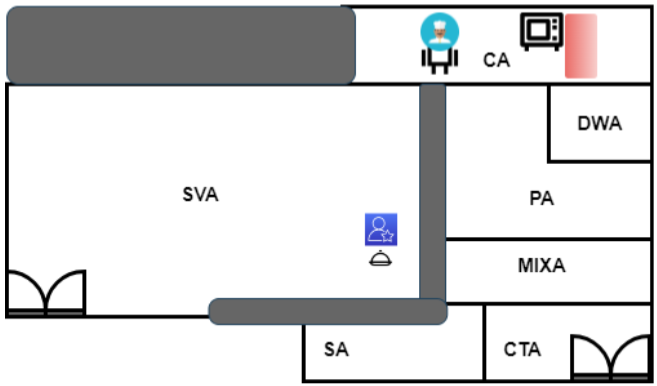
\includegraphics[width=0.5\linewidth]{restaurante.png}
  \caption{Restaurant structure. Gray areas means that the robot can not move in these areas.}
  \label{fig:restaurant}
\end{figure}

Subsequently, we will introduce the common predicates and actions used across all three scenarios considered in this project.
\subsection{Basic problem}\label{subsec:basic}
It consists of the preparation of a simple sushi recipe. The ingredients were placed in the STA, and each of them had specific 
requirements to be prepared (e.g., rice needed to be mixed and cooked, fish needed to be cut). Each action was carried out in the 
area designated for it, and the final goal was to plate the dish in the serving area and return all the tools used to their original
 place, clean and ready for future use.

 The predicates used are listed below.
\begin{itemize}
  \item $ (\text{robot-at } ?r \text{ - robot } ?loc \text{ - location}) $: Represents the location of a specific robot 'r' in an area of the kitchen 'loc'.
  \item $ (\text{ingredient-at } ?\text{ingredient - ingredient } ?\text{loc - location}) $: This predicate signifies the presence of an 'ingredient' in an area 'loc'.
  \item $ (\text{tool-at } ?\text{tool - tool } ?\text{loc - location}) $: This predicate indicates that the instrument 'tool' is in the area of the kitchen 'loc'.
  \item $ (\text{ingredient-prepared } ?\text{ingredient - ingredient}) $: This predicate indicates that the ingredient 'ingredient' has been successfully prepared.
  \item $ (\text{dish-assembled } ?\text{dish - dish}) $: Indicates that the dish 'dish' has been assembled from its ingredients.
  \item $ (\text{dish-plated } ?\text{dish - dish } ?\text{loc - location}) $: Denotes that the dish 'dish' has been plated and placed at location 'loc'.
  \item $ (\text{tool-clean } ?\text{tool - tool}) $: This predicate denotes that the tool 'tool' is clean.
  \item $ (\text{holding-ingredient } ?\text{r - robot } ?\text{ingredient - ingredient}) $: Indicates that the robot 'r' is holding the ingredient 'ingredient'.
  \item $ (\text{holding-dish } ?\text{r - robot } ?\text{dish - dish}) $: Indicates that the robot 'r' is holding the assembled dish 'dish'.
  \item $ (\text{holding-tool } ?\text{r - robot } ?\text{tool - tool}) $: Indicates that the robot 'r' is holding the tool 'tool'.
  \item $ (\text{adjacent } ?\text{loc1 - location } ?\text{loc2 - location}) $: Indicates that the kitchen areas 'loc1' and 'loc2' are adjacent.
  \item $ (\text{used-in } ?\text{ingredient - ingredient } ?\text{dish - dish}) $: This predicate represents if the ingredient 'ingredient' has been used to prepare the dish 'dish'.
  \item $ (\text{need-mix } ?\text{ingredient - ingredient}) $: Denotes that the ingredient 'ingredient' requires mixing.
  \item $ (\text{need-cook } ?\text{ingredient - ingredient}) $: Denotes that the ingredient 'ingredient' requires cooking.
  \item $ (\text{need-cut } ?\text{ingredient - ingredient}) $: Denotes that the ingredient 'ingredient' requires cutting.
\end{itemize}
The actions specified are outlined hereafter.
\begin{itemize}
    \item \textbf{pick-up-ingredient:} The robot picks up an ingredient at a specified location.
    \item \textbf{pick-up-tool:} The robot picks up a tool at a specified location.
    \item \textbf{move:} The robot moves from one location to an adjacent location.
    \item \textbf{drop-ingredient:} The robot drops the ingredient it is holding at a specified location.
    \item \textbf{drop-tool:} The robot drops the tool it is holding at a specified location.
    \item \textbf{mix:} The robot mixes an ingredient (e.i. rice) at the mixing area (MIXA), provided the ingredient needs mixing and is not already prepared.
    \item \textbf{cook:} The robot cooks an ingredient (e.i. rice) at the cooking area (CA), provided it has been mixed and needs cooking.
    \item \textbf{cut:} The robot cuts an ingredient at the cutting area (CTA) using a clean tool, provided the ingredient needs cutting.
    \item \textbf{clean-tool:} The robot cleans a tool in the dishwashing area (DWA).
    \item \textbf{assemble-dish:} The robot assembles a dish using prepared ingredients at a specified location.
    \item \textbf{carrying-dish:} The robot carries an assembled dish, provided it is not already holding any other items.
    \item \textbf{plate-dish:} The robot plates an assembled dish at the serving area (SVA).
\end{itemize}

\subsection{Substitution problem}
In this scenario, the same sushi recipe as before needs to be plated; nevertheless, an ingredient used in this dish is missing at the 
STA. Other ingredients were available, and several predicates were given to the robot to inform it about possible substitutions. 
The robot was able to examine the available ingredients and decide whether to make a substitution in order to complete its task. 

The same predicates and actions as those described for the \textbf{basic problem} in subsection \ref{subsec:basic} were used. 
However, one additional predicate and action were included in this PDDL domain to account for the new problem.
\\ \\ 
Additional predicate:
\begin{itemize}
  \item $ (\text{replaceable } ?ingredient1  \text{ - ingredient }  ?ingredient2 \text{ - ingredient }  ?dish  \text{ - dish}) $: Represents that 'ingredient1' can be replaced by 'ingredient2' in the preparation of 'dish'.
\end{itemize}
Additional action:
\begin{itemize}
  \item \textbf{substitution-decision:} The robot makes the decision of changing the 'ingredient1', that is used in the preparation of 
  a dish, by 'ingredient2' when the first one is missing and the second one is suitable for the change.
\end{itemize}

\subsection{Priorization order problem}

\section{Results}
In all the scenarios described in the previous section, the results were obtained using a PDDL planner implemented in Julia. 
Specifically, the A* search algorithm was implemented. The planner initializes the problem state using the initstate function and 
defines the goals using MinStepsGoal, optimizing for minimal steps to achieve the objectives, while the planning process employs an A$*$ 
planner (AStarPlanner) with the HAddR heuristic to guide the search.


The implementation of Julia was mandatory due to...


The final path obtained for each case can be seen in ... 
\section{Discusion}
In this section, it is analyzed the plans obtained in each scenario and how they were achieved. In order to provide a insight into the 
efficiency and complexity of the searching process, several key performance parameters were analyzed, as it is shown in Table \ref{tab:tabla}. 

\begin{table}[H]
    \begin{tabular}{|l|c|c|c|}
    \hline
    Problem         & Basic & Substitution & Priorization order \\ \hline
    Plan length     &  41     &    42          &                    \\ \hline
    Expanded states &    33413   &     34710         &                    \\ \hline
    Search time (s)    & 36.0221934      &    58.560908       &                    \\ \hline
    Total time (s)     &   36.0221938     &     58.5609156           &                    \\ \hline
    \end{tabular}\label{tab:tabla}
    \caption{Performance of the planners across different test cases.}
\end{table}

\section{Conclusion}
Hola\cite{key}

\bibliographystyle{plain}
\bibliography{bibliography.bib}

\end{document}